%-------------------------------------------------------------------------------
%	PACKAGES AND OTHER DOCUMENT CONFIGURATIONS
%-------------------------------------------------------------------------------
\documentclass{article}% A4 paper and 11pt font size

\usepackage{amsmath,amsfonts,amsthm} % Math packages
\usepackage{mcode} %Include Matlab code
\usepackage{graphicx}
\usepackage{float}
\usepackage{caption}
\usepackage{subcaption}
\usepackage{fullpage}
\usepackage{url}
%-------------------------------------------------------------------------------
%	TITLE SECTION
%-------------------------------------------------------------------------------

\title{
\textsc{Artificial Neural Networks} \\ [25pt]
\huge Benchmark Problem Report \\ % The assignment title
}

\author{Antonio Peters} % Your name

\date{\today} % Today's date or a custom date

%%%%%%%%%%%%%%%%%%%%%%%%%%%%%%%%%%%%%%%%%%%%%%%%%%%%%%%%%%%%%%%%%%%%%%%
%DOCUMENT
%%%%%%%%%%%%%%%%%%%%%%%%%%%%%%%%%%%%%%%%%%%%%%%%%%%%%%%%%%%%%%%%%%%%%%%
\begin{document}
\maketitle % Print the title
%%%%%%%%%%%%%%%%%%%%%%%%%%%%%%%%%%%%%%%%%%%%%%%%%%%%%%%%%%%%%%%%%%%%%%%
\section{Introduction}
For this report, all data sets are obtained from \url{https://archive.ics.uci.edu/ml/datasets.html}. The code run for this report is written in the MATLAB programming language. All code can be accessed in their respective folders in the same directory as this document.
%%%%%%%%%%%%%%%%%%%%%%%%%%%%%%%%%%%%%%%%%%%%%%%%%%%%%%%%%%%%%%%%%%%%%%%
\section{Mushrooms}
The mushroom classification set seeks to classify mushrooms into two groups, poisonous and edible. It does this by looking at 22 input parameters: cap shape, cap surface, cap color, bruises, odour, gill attachment, gill spacing, gill size, gill color, stalk shape, stalk root, stalk surface above ring, stalk surface below ring, stalk color above ring, stalk color below ring, veil-type, veil color, ring number, ring type, spore print color, population and habitat. Before starting to write the code for the net, we first remove $49$ rows of the data set randomly and store in a separate data file for testing once our net has been finalised.
\\
\\
We begin by importing the data and normalising it so it can be used as input into the net. The data is presented as a series of characters with 23 characters to a row, each separated by a comma, this represents the 22 parameters and the corresponding result. The data is first separated into a $22 \times n$ matrix for the input and a vector of $n$ length for the output. Each element of the input is then converted to its corresponding ASCII value and $97$ is subtracted so that $a=0,b=1,...,z=25$ for each element. In the output vector, there are only two possible answers, $p$ and $e$ for poisonous and edible, these are translated to $0$ and $1$ respectively. It has been stated by the supplier of the data that the dataset is incomplete, as such there are elements of the input data which are labelled as $?$, these then correspond to a negative value in the transformed input matrix, therefore any rows containing negative values are removed and their corresponding output value is also removed from the output vector as this could mislead our network.
\\
\\
The data is then split into training and testing sets in a ratio of $3:1$. A 3-layer feed-forward neural network will be used to train on the training data. A triple nested for-loop is generated to iterate through the number of neurons for each of the net's layers from $1$ to $20$. From this, the best net is selected and stored, the criteria for the best network is based resulting in the highest $r^2$ and Correlation Coefficient values determined by simulating the network on the remaining test data. Once a best network has been found, its error is determined and plotted as shown in Figure \ref{fig:mushtrain}.
\begin{figure}[H]
\centering
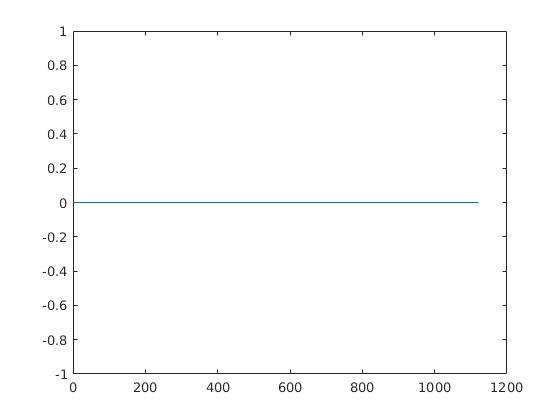
\includegraphics[scale=0.5]{Images/mushtrain.jpg}
\caption{Mushroom best NN test error.}
\label{fig:mushtrain}
\end{figure}
The optimal net was found to be three layers each with only one neuron, the resulting correlation coefficient and $r^2$ values were determined and both were found to be $1$.
\\
\\
Now that we have the best net for our given data set, we can simulate on the reserved $49$ element as a final validation test. We begin this process by normalising the data by the same method as the training set. We then simulate on this normalised data and plot the output. The data is presented with the actual output as blue circles and the simulated output as red asterisks, this can be seen in Figure \ref{fig:mushtest}.
\begin{figure}[H]
\centering
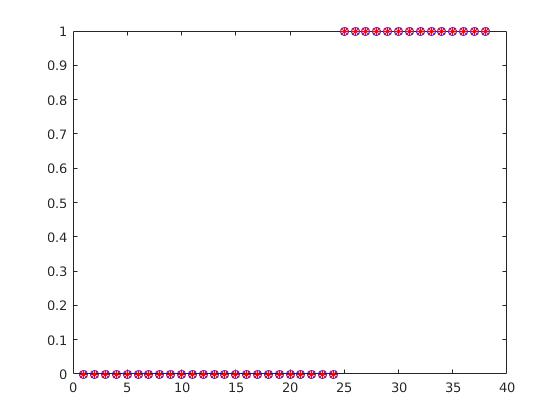
\includegraphics[scale=0.5]{Images/mushtest.jpg}
\caption{Mushroom net on the reserved test data.}
\label{fig:mushtest}
\end{figure}
This shows that our neural net trained well on the training data and is able to categorize new data perfectly.
%%%%%%%%%%%%%%%%%%%%%%%%%%%%%%%%%%%%%%%%%%%%%%%%%%%%%%%%%%%%%%%%%%%%%%%
\section{Ionosphere}
The ionosphere classification set seeks to classify weather into two groups, good or bad. It does this by looking at 34 continuous input parameters. Before starting to write the code for the net, we first remove $11$ rows of the data set randomly and store in a separate data file for testing once our net has been finalised.
\\
\\
We begin by importing the data and normalising it so it can be used as input into the net. The data is presented as a series of $34$ double values and a single character to a row, each separated by a comma, this represents the $34$ parameters and the corresponding result. The data is first separated into a $34 \times n$ matrix for the input and a vector of $n$ length for the output. Each element of the output vector is translated to $0$ or $1$ for bad $(b)$ or good $(g)$ weather respectively.
\\
\\
The data is then split into training and testing sets in a ratio of $3:1$. A 3-layer feed-forward neural network will be used to train on the training data. A triple nested for-loop is generated to iterate through the number of neurons for each of the net's layers from $1$ to $20$. From this, the best net is selected and stored, the criteria for the best network is based resulting in the highest $r^2$ and Correlation Coefficient values determined by simulating the network on the remaining test data. Once a best network has been found, its error is determined and plotted as shown in Figure \ref{fig:iontrain}.
\begin{figure}[H]
\centering
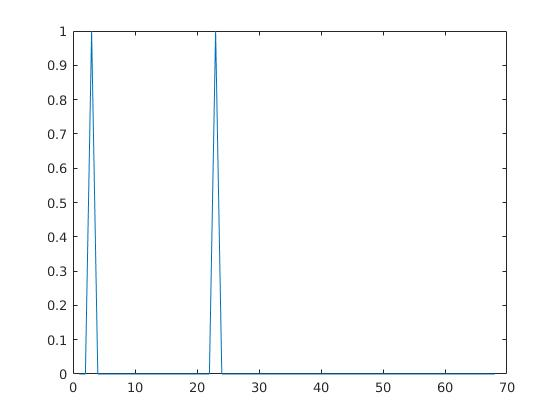
\includegraphics[scale=0.5]{Images/iontrain.jpg}
\caption{Ionosphere best NN test error.}
\label{fig:iontrain}
\end{figure}
From this, it can be seen that the net trains the data with only two incorrect classifications for the test set. The resulting $r^2$ and correlation coefficient values were $0.8735$ and $0.9396$ respectively which indicates a strong relationship between the output and the simulation output for the data set. The optimal net consists of 19, 7 and 7 neurons at each layer.
\\
\\
Now that we have the best net for our given data set, we can simulate on the reserved $11$ element as a final validation test. We begin this process by normalising the data by the same method as the training set. We then simulate on this normalised data and plot the output. The data is presented with the actual output as blue circles and the simulated output as red asterisks, this can be seen in Figure \ref{fig:iontest}.
\begin{figure}[H]
\centering
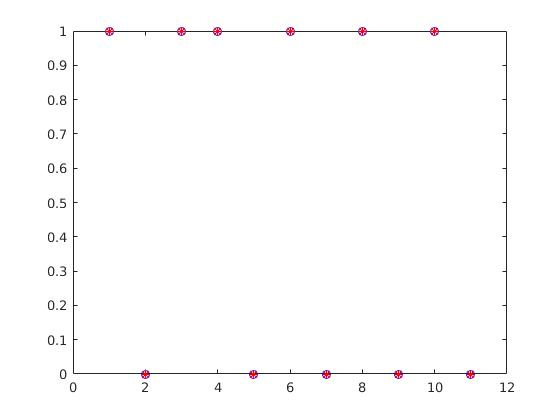
\includegraphics[scale=0.5]{Images/iontest.jpg}
\caption{Ionosphere net on the reserved test data.}
\label{fig:iontest}
\end{figure}
From this it, it can be seen that the data classifies the data perfectly, though this is a small data set. Possible reasons as to why the data is not perfectly classified in the training test set is possibly due to the fact that the classification of 'good' or 'bad' weather is subjective.
%%%%%%%%%%%%%%%%%%%%%%%%%%%%%%%%%%%%%%%%%%%%%%%%%%%%%%%%%%%%%%%%%%%%%%%
\section{Energy Efficiency}
The energy efficiency problem set seeks to determine the heating and cooling load of a room. It does this by looking at 8 continuous input parameters: compactness, surface area, wall area, roof area, overall height, orientation, glazing area and glazing area distribution. Before starting to write the code for the net, we first remove $29$ rows of the data set randomly and store in a separate data file for testing once our net has been finalised.
\\
\\
We begin by importing the data and normalising it so it can be used as input into the net. The data is presented as a series of $10$ double values to a row, each separated by a comma, this represents the $8$ parameters and their corresponding $2$ result. The data is first separated into a $8 \times n$ matrix for the input and a $2 \times n$ matrix for the output.
\\
\\
The data is then split into training and testing sets in a ratio of $2:3$.  From the training set, the greatest distance between elements is found and is used to determine the spread of the data. From this spread, 11 spreads are generated, all within range of the generated spread. Using each spread, a radial basis network is generated to calculate the output. The nets are then tested and the best testing net is then chosen. The best net is again determined by the highest $r^2$ and Correlation Coefficient values. The output for this net can be seen in Figures  \ref{fig:enetrain1} and \ref{fig:enetrain2}.
\begin{figure}[H]
\centering
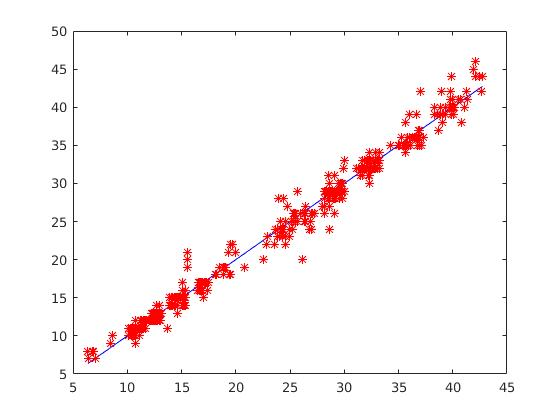
\includegraphics[scale=0.5]{Images/enetrain1.jpg}
\caption{Heating load best NN test error.}
\label{fig:enetrain1}
\end{figure}
\begin{figure}[H]
\centering
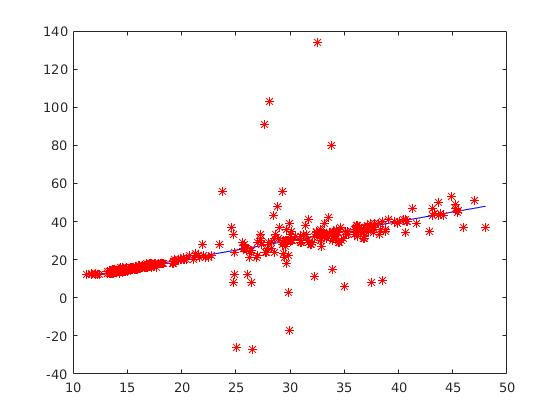
\includegraphics[scale=0.5]{Images/enetrain2.jpg}
\caption{Cooling load best NN test error.}
\label{fig:enetrain2}
\end{figure}
The best spread for the data was found to be $15.808692849068090$. The corresponding $r^2$ values were $0.9866$ for heating and $0.0142$ for cooling and a correlation coefficient of $0.8218$. From the figures and the $r^2$ values it can be seen that the data approximates the heating data much better than the cooling.
\\
\\
Now that we have the best net for our given data set, we can simulate on the reserved $11$ element as a final validation test. We begin this process by normalising the data by the same method as the training set. We then simulate on this normalised data and plot the output. The data is presented with the actual output as blue circles and the simulated output as red asterisks, this can be seen in Figure \ref{fig:enetest1} and \ref{fig:enetest2}.
\begin{figure}[H]
\centering
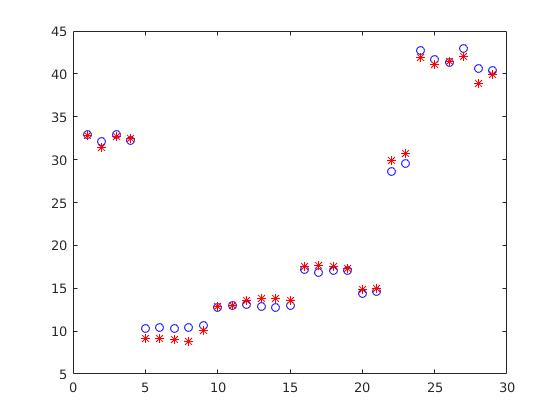
\includegraphics[scale=0.5]{Images/enetest1.jpg}
\caption{Heating load net on the reserved test data.}
\label{fig:enetest1}
\end{figure}
\begin{figure}[H]
\centering
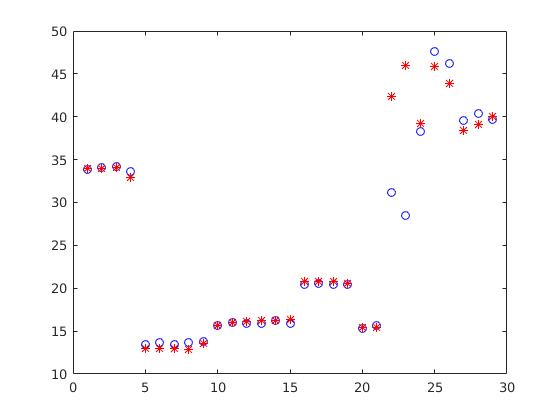
\includegraphics[scale=0.5]{Images/enetest2.jpg}
\caption{Cooling load net on the reserved test data.}
\label{fig:enetest2}
\end{figure}
From these images it cam be seen that the net approximates the heating data very closely to the real data but fails to approximate correctly for some of the cooling data. 
%%%%%%%%%%%%%%%%%%%%%%%%%%%%%%%%%%%%%%%%%%%%%%%%%%%%%%%%%%%%%%%%%%%%%%%
\section{Seeds}
The seed classification set seeks to classify seeds into one of three types of wheat, Kama, Rosa or Canadian. It does this by looking at 7 continuous geometric input parameters: the area of the seed, the perimeter of the seed, the compactness of the seed, the length of kernel, the width of kernel, the asymmetry coefficient and the length of kernel groove. Before starting to write the code for the net, we first remove $23$ rows of the data set randomly and store in a separate data file for testing once our net has been finalised.
\\
\\
We begin by importing the data and normalising it so it can be used as input into the net. The data is presented as a series of $7$ double values and a single integer of value 1, 2 or 3, each separated by a comma, this represents the $7$ parameters and the corresponding result. The data is first separated into a $7 \times n$ matrix for the input and a vector of $n$ length for the output. Each element of the output vector is then converted to one of three basis vectors, to ensure that the net does not mistake the seed type from being a continuous data set, this then forms our output into a $3 \times n$ matrix.
\\
\\
The data is then split into training and testing sets in a ratio of $3:1$. A 3-layer feed-forward neural network will be used to train on the training data. A triple nested for-loop is generated to iterate through the number of neurons for each of the net's layers from $1$ to $20$. From this, the best net is selected and stored, the criteria for the best network is based resulting in the highest $r^2$ and Correlation Coefficient values determined by simulating the network on the remaining test data. Once a best network has been found, its result is rounded to form a vector of integers and is then converted back to integers so that the error can be determined and plotted with the actual output as blue circles and the simulated output as red asterisks in Figure \ref{fig:seedtrain}.
\begin{figure}[H]
\centering
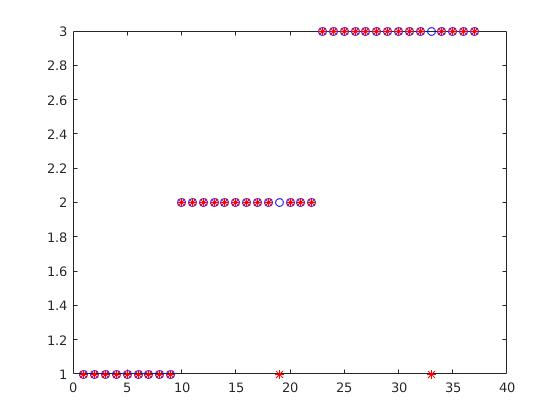
\includegraphics[scale=0.5]{Images/seedtrain.jpg}
\caption{Seeds best NN test error.}
\label{fig:seedtrain}
\end{figure}
From this, it can be seen that the net trains the data with only two incorrect classifications for the test set. The resulting $r^2$ values were $0.706349206349206$, $0.881410256410257$ and $0.887878787878788$ and a correlation coefficient of $0.9189$ which indicates a strong relationship between the output and the simulation output for the data set. The optimal net consists of 20, 20 and 20 neurons at each layer.
\\
\\
Now that we have the best net for our given data set, we can simulate on the reserved $23$ element as a final validation test. We begin this process by normalising the data by the same method as the training set. We then simulate on this normalised data and plot the output. The data is presented with the actual output as blue circles and the simulated output as red asterisks, this can be seen in Figure \ref{fig:seedtest}.
\begin{figure}[H]
\centering
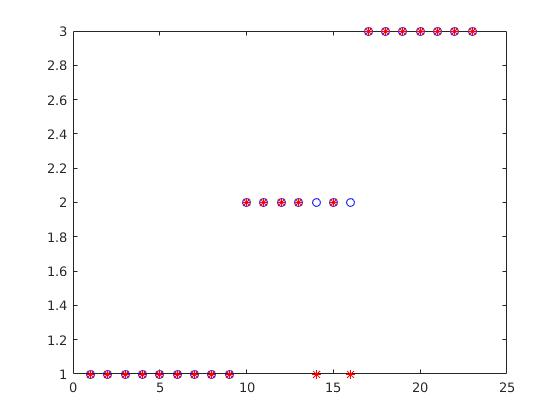
\includegraphics[scale=0.5]{Images/seedtest.jpg}
\caption{Seed net on the reserved test data.}
\label{fig:seedtest}
\end{figure}
From this it, it can be seen that the data classifies the data very well with only two incorrect classifications, though this is a small data set.
%%%%%%%%%%%%%%%%%%%%%%%%%%%%%%%%%%%%%%%%%%%%%%%%%%%%%%%%%%%%%%%%%%%%%%%
\section{Concrete}
The concrete strength approximation set seeks to approximate the compressive strength of concrete. It does this by looking at 8 continuous input parameters, namely the amounts of: cement, blast furnace slag, fly ash, water, superplasticizer, coarse aggregate, fine aggregate and the age of the concrete. Before starting to write the code for the net, we first remove $20$ rows of the data set randomly and store in a separate data file for testing once our net has been finalised.
\\
\\
We begin by importing the data and normalising it so it can be used as input into the net. The data is presented as a series of $9$ double values, each separated by a comma, this represents the $8$ parameters and the corresponding result. The data is first separated into a $8 \times n$ matrix for the input and a vector of $n$ length for the output.
\\
\\
The data is then split into training and testing sets in a ratio of $3:1$. A 3-layer feed-forward neural network will be used to train on the training data. A triple nested for-loop is generated to iterate through the number of neurons for each of the net's layers from $1$ to $20$. From this, the best net is selected and stored, the criteria for the best network is based resulting in the highest $r^2$ and Correlation Coefficient values determined by simulating the network on the remaining test data. Once a best network has been found, the error on the test set can be determined by observing Figure \ref{fig:contrain}, where the actual output is represented by a blue line and the simulated output as red asterisks.
\begin{figure}[H]
\centering
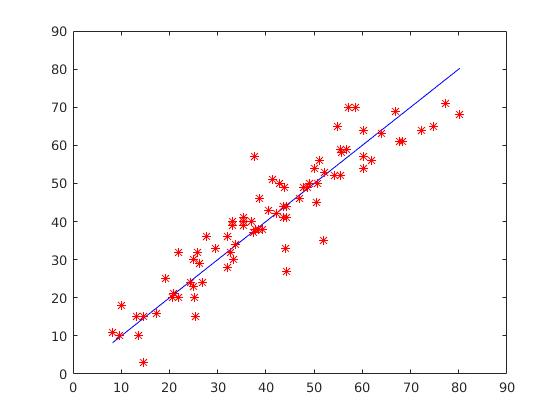
\includegraphics[scale=0.5]{Images/contrain.jpg}
\caption{Concrete best NN test error.}
\label{fig:contrain}
\end{figure}
From this we can see that while the simulation is approximately correct, it does not perfectly match the output. The net generates a correlation coefficient of 0.9304 and a $r^2$ value of $0.8632$, showing that the data has adequate linear correlation. The network has 20, 4 and 3 neurons per layer.
\\
\\
Now that we have the best net for our given data set, we can simulate on the reserved $20$ element as a final validation test. We begin this process by normalising the data by the same method as the training set. We then simulate on this normalised data and plot the output. The data is presented with the actual output as blue circles and the simulated output as red asterisks, this can be seen in Figure \ref{fig:contest}.
\begin{figure}[H]
\centering
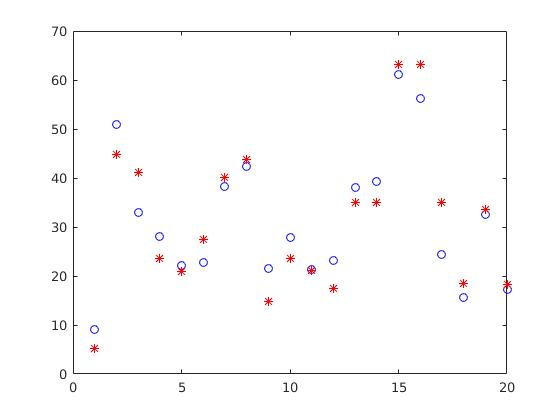
\includegraphics[scale=0.45]{Images/contest.jpg}
\caption{Concrete net on the reserved test data.}
\label{fig:contest}
\end{figure}
From this it can be seen that the simulation approximates the output to within $10$ of the exact output. While this is adequate for a general approximation, it cannot be said that this is the optimal net for training on this data.
%%%%%%%%%%%%%%%%%%%%%%%%%%%%%%%%%%%%%%%%%%%%%%%%%%%%%%%%%%%%%%%%%%%%%%%
\end{document} 